\chapter[Revisão Sistemática]{Revisão Sistemática}

    Este capítulo apresenta conceitos pertinentes aos principais tópicos que serão abordados
    nesse TCC. Os tópicos abordados são, \textit{Hadoop, MapReduce, Spark, Impala, HBase e
    Cloudera.}

    \section{Hadoop}

            O \textit{Hadoop} foi criado por Doug Cutting, o mesmo criador do Apache Lucene, a biblioteca de busca
            textual \cite{white2015}. O \textit{Hadoop} é composto por dois componentes principais, o HDFS que é
            um sistema de arquivos para ser usado em \textit{cluster}, e o \textit{MapReduce} que é responsável
            pelo processamento dos dados armazenados no sistema de arquivos. O \textit{Hadoop} em comparação
            com outros sistemas de arquivos distribuídos possui é um sistema tolerante a falhas críticas, e foi
            desenvolvido para rodar em máquinas de baixo custo com um modelo de programação simples
            \cite{alam2014}. Segundo \citeonline{alam2014}, o \textit{Hadoop} cobre quase todos os aspectos dos
            paradigmas de sistemas distribuídos como confiabilidade, eficiência, disponibilidade, acurácia e segurança.

        \subsection{Hadoop Distributed File System}

            O HDFS é um sistema de arquivos distribuídos desenvolvido para armazenar arquivos muito grandes
            com um padrão de fluxo de dados, que funcionam dentro de um \textit{cluster} de máquinas de baixo
            custo \cite{white2015}.

            As suas principais características são, lotes de grandes arquivos a serem processados, o fluxo de acesso
            de dados em que o sistema escreve uma vez e lê várias vezes em determinado padrão e pôr fim a baixa
            necessidade de uma estrutura de ponta, pois o próprio sistema já fornece quase todos os aspectos dos
            paradigmas que os sistemas distribuídos tentam cobrir, logo foi desenvolvido para rodar em máquinas de
            baixo custo (computadores domésticos são exemplos de máquinas de baixo custo), o sistema se utiliza de
            implementações contra falhas críticas para, caso um \textit{node} venha a falhar o HDFS ainda continue
            trabalhando sem interrupções \cite{white2015}.

            \subsubsection{Bloco de Dados}

                O conceito de bloco de dados, se refere ao \textit{container} que será utilizado para o armazenamento
                dos dados. Este \textit{container} possui um tamanho padrão que pode ser definido nas configurações
                do HDFS dependendo da necessidade do cliente. O bloco de dados então é armazenado ao longo do
                \textit{cluster} e suas referências são guardadas.

                O motivo pelo qual se dá preferência a arquivos muito grandes, é pela necessidade de dividir esses
                arquivos em blocos, para que encaixem nos \textit{containers}. Para \citeonline{white2015}, ter
                uma abstração de bloco para um \textit{Distributed Filesystem} (DFS) pode trazer uma série de
                benefícios como o caso de um arquivo ser maior que o disco, então existe a vantagem de ter vários
                discos em \textit{cluster}.

                Outra vantagem, está na abstração dos blocos ao invés de arquivos, e isso simplifica o armazenamento.
                O subsistema de armazenamento usa blocos de dados para simplificar o gerenciamento de armazenamento,
                pois como os blocos possuem tamanhos fixos, fica fácil determinar a alocação dos blocos ao longo dos
                discos \cite{white2015}.

                Não existe necessidade de preocupação com os metadados levando em consideração que os blocos são
                apenas pedaços de dados que são armazenados, já os arquivos de metadados tais como informações sobre
                permissões não precisam ser armazenados com os blocos, pois existe outro sistema que trata dos metadados
                separadamente \cite{shvachko2010}.

                \begin{figure}[ht!]
                    \centering
                    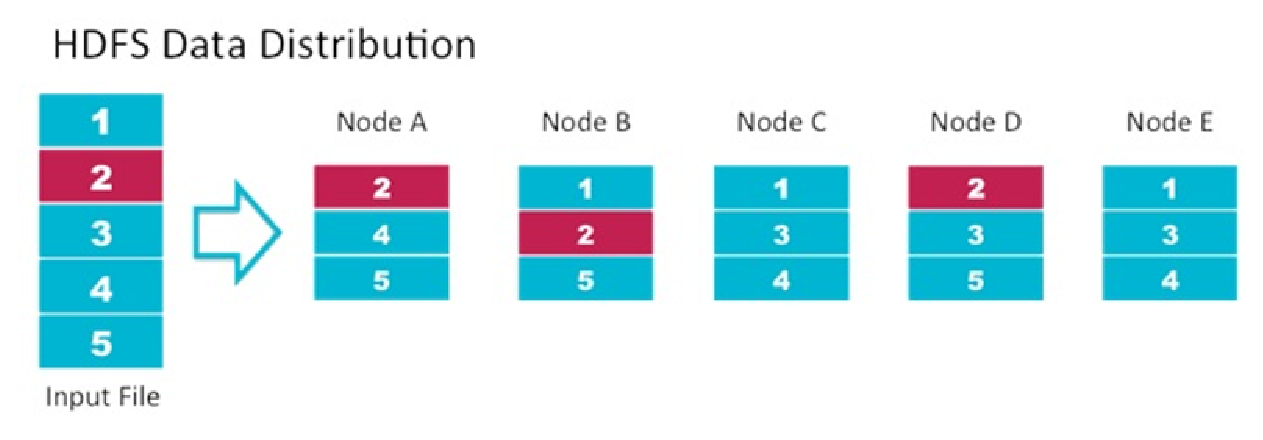
\includegraphics[keepaspectratio=true,scale=0.75]
                        {figuras/figura1.eps}
                    \caption[Distribuição em Blocos no HDFS]{Distribuição em Blocos no HDFS
                    \protect\linebreak Fonte: \citeonline{hadoopexample}}
                    \label{figura1}
                \end{figure}

                Com a replicação dos dados, temos a garantia de que mesmo que um \textit{node} venha a falhar o dado
                não será perdido, garantindo a proteção contra falhas críticas e disponibilidade. Essa replicação é realizada
                por padrão de distribuição em até três maquinas, mas essa configuração pode ser alterada dependendo da
                necessidade do cliente para garantir a integridade de seus dados.

            \subsubsection{Arquitetura HDFS}

                Em um cluster de HDFS, existem dois tipos de \textit{nodes} operantes no caso o: \textit{namenode} (\textit{master})
                e um certo número de \textit{datanodes} (trabalhadores). O \textit{namenode} gerencia o \textit{namespace} e
                mantêm a arvore do sistema de arquivos e dos metadados para todos os arquivos e diretórios na estrutura. Essa
                informação é armazenada no disco local em forma de dois arquivos, a imagem do \textit{namespace} e o log de edição.
                De acordo com \citeonline{shvachko2010}, o \textit{namenode} conhece em quais \textit{datanodes}  determinado
                arquivo está localizado, porém ele não reconstrói o local, por que essa informação é reconstruída a partir dos
                \textit{datanodes} quando o sistema inicia \cite{white2015}.

                O \textit{client} acessa o sistema de arquivos em nome do usuário, se comunicando com o \textit{namenode} e
                \textit{datanodes}. A interface do \textit{client} é similar ao \textit{Portable Operating System Interface} (sistema
                que o kernel do Linux usa), logo o usuário não precisa saber sobre as funções do \textit{namenode} e
                \textit{datanodes} em específico.

                \begin{figure}[ht!]
                    \centering
                    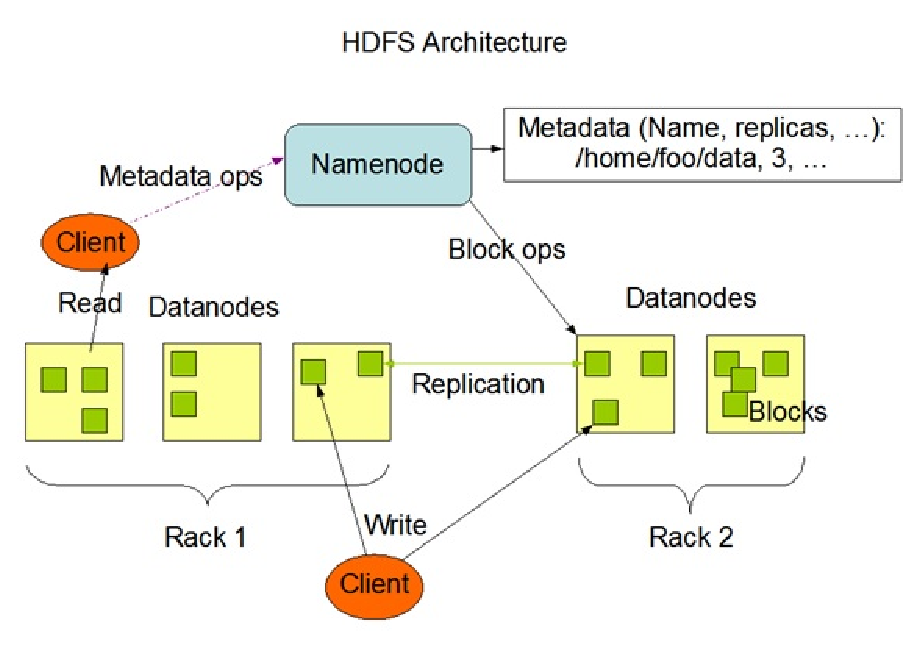
\includegraphics[keepaspectratio=true,scale=0.75]
                        {figuras/figura2.eps}
                    \caption[Arquitetura do HDFS]{Arquitetura do HDFS
                    \protect\linebreak Fonte: \citeonline{hadoopapache}}
                    \label{figura2}
                \end{figure}

                Na figura \ref{figura2}, temos a visualização da arquitetura do HDFS, o \textit{namenode} manipula
                os metadados que são essenciais para a aplicação \textit{client}, nele temos dados do \textit{namespace}
                e o número de réplicas bem como outras informações a mais, e com o mapeamento desses dados a aplicação
                consegue recuperar o dado que precisa nos \textit{datanodes} referenciados.

            \subsubsection{Processo de Leitura e Escrita}

                Quando uma aplicação vai ler um arquivo, o HDFS \textit{client} pergunta ao \textit{namenode} pela lista
                de \textit{datanodes} que guardam as réplicas de determinado bloco do arquivo. Só então a aplicação
                comunica-se com o \textit{datanode} diretamente e requisita a transferência de determinado bloco. É
                possível visualizar esse processo de forma detalhada na figura 3, o qual temos uma aplicação do HDFS
                em cima de uma \textit{Java Virtual Machine} (JVM) que se comunica com os \textit{nodes} em determinada
                ordem, para obter um determinado arquivo \cite{shvachko2010}.

                Já quando a aplicação escreve, ele pergunta ao \textit{namenode} para que escolha os \textit{datanodes}
                que serão utilizado para armazenar o primeiro bloco do arquivo, então o \textit{client} organiza uma
                \textit{pipeline} de \textit{node} para \textit{node} e envia os dados. Quando o primeiro bloco é preenchido,
                o \textit{client} faz uma nova requisição por novos \textit{datanodes} a serem escolhidos para guardarem
                as réplicas do próximo bloco. Esse mesmo processo é possível de ser visualizado na figura 4 com detalhes
                \cite{shvachko2010}.

                \begin{figure}[ht!]
                    \centering
                    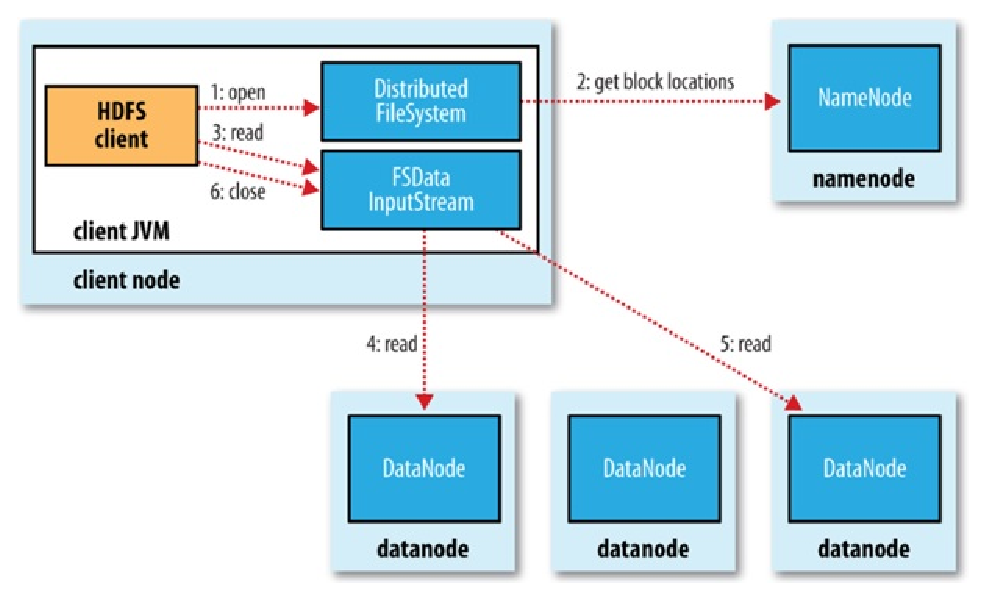
\includegraphics[keepaspectratio=true,scale=0.75]
                        {figuras/figura3.eps}
                    \caption[Processo de Leitura no HDFS]{Processo de Leitura no HDFS
                    \protect\linebreak Fonte: \citeonline{white2015}}
                    \label{figura3}
                \end{figure}

                \begin{figure}[ht!]
                    \centering
                    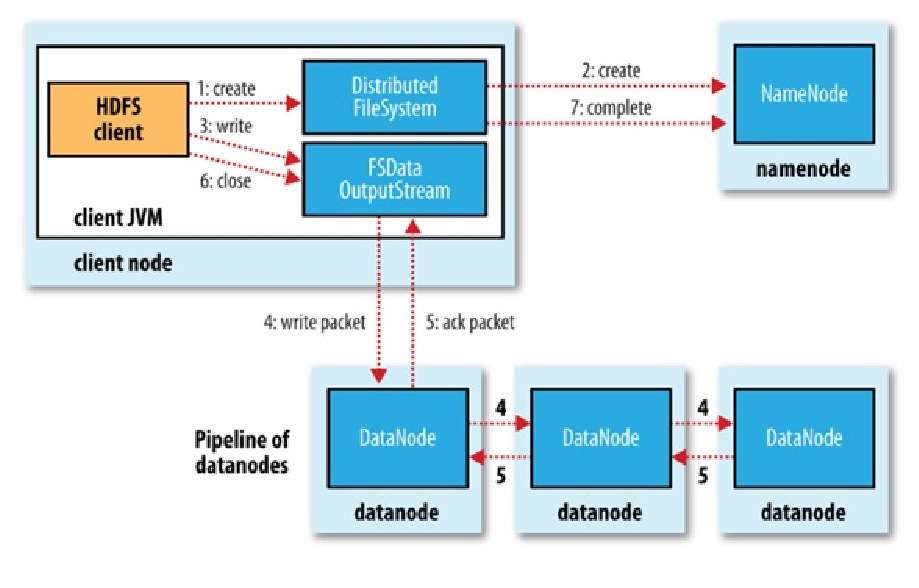
\includegraphics[keepaspectratio=true,scale=0.75]
                        {figuras/figura4.eps}
                    \caption[Processo de Escrita no HDFS]{Processo de Escrita no HDFS
                    \protect\linebreak Fonte: \citeonline{white2015}}
                    \label{figura4}
                \end{figure}

        \subsection{MapReduce}

            O desenvolvimento do \textit{MapReduce} surgiu de uma necessidade de processamento de uma grande
            quantidade de dados brutos, com o objetivo  de computar diversos tipos de dados derivados, como índices,
            representações gráficas acerca de determinados dados, sumarização, dentre outras \textit{queries} frequentes
            usadas no dia-a-dia. Porém os dados de entrada são geralmente grandes e computacionalmente precisam ser
            distribuídos ao longo de milhares de máquinas, para que seja possível de terminar em uma quantidade de
            tempo razoável \cite{dean2008}.

            De acordo com \citeonline{dean2008}, o \textit{MapReduce} foi desenvolvido em resposta a complexidade
            que se tem para processamento de dados em lote em uma arquitetura distribuída. Então essa camada de
            abstração permite expressar uma computação mais simples, mas que por baixo, abstrai detalhes de computação
            paralela, tolerância a falhas, distribuição de dados e balanceamento de carga só que em uma biblioteca.

            O \textit{MapReduce} funciona quebrando o processo em duas fases, a fase de \textit{map} e a fase de
            \textit{reduce}. Cada fase tem um par de \{chave,valor\} como entrada e saída. O programador também
            especifica as duas funções, a função de \textit{map} e a função de \textit{reduce} \cite{white2015}.

            A função \textit{map} escrita pelo usuário, precisa de um par na entrada e produz um intervalo de pares de
            \{chave,valor\}. A biblioteca agrupa juntamente com todos os valores intermediários associados com a mesma
            chave intermediária e repassa para a função \textit{reduce}. Já a função \textit{reduce} aceita uma chave
            intermediária e um intervalor de valores para aquela chave. Esses valores são agrupados para forma um
            intervalo menor ainda de valores, tipicamente apenas zeros ou uma entrada de valores produzidos por
            invocação do \textit{reduce}. Esses valores intermediários são produzidos pelas funções \textit{reduce}
            do usuário que vão sendo iteradas. Isto nos permite manejar a lista de valores que são muito grandes
            para caber na memória \cite{dean2008}.

            De acordo com \citeonline{white2015} o \textit{MapReduce job} é uma unidade de trabalho que a
            aplicação deseja que seja processada, e consiste em uma entrada de dados, a definição do
            \textit{MapReduce} programado e a configuração das informações. O Hadoop executa o \textit{job}
            dividindo ele em dois tipos de tarefas, as chamadas \textit{map tasks} e \textit{reduce tasks}.
            Essas tarefas são organizadas usando o YARN (\textit{Yet Another Resource Negotiator}) e são
            executadas nos \textit{nodes} do cluster, e se a tarefa falha, ela será automaticamente reorganizada
            para a fila de execução em um \textit{node} diferente. Na figura \ref{figura5} temos a ilustração no
            processo \textit{shuffle} e \textit{sort}  que é um processo que garante que toda entrada para cada
            \textit{reduce} tenha uma chave, e que valor seja repassado a saída do \textit{map} para as
            entradas das funções \textit{reduce}\cite{white2015}.

            \begin{figure}[ht!]
                    \centering
                    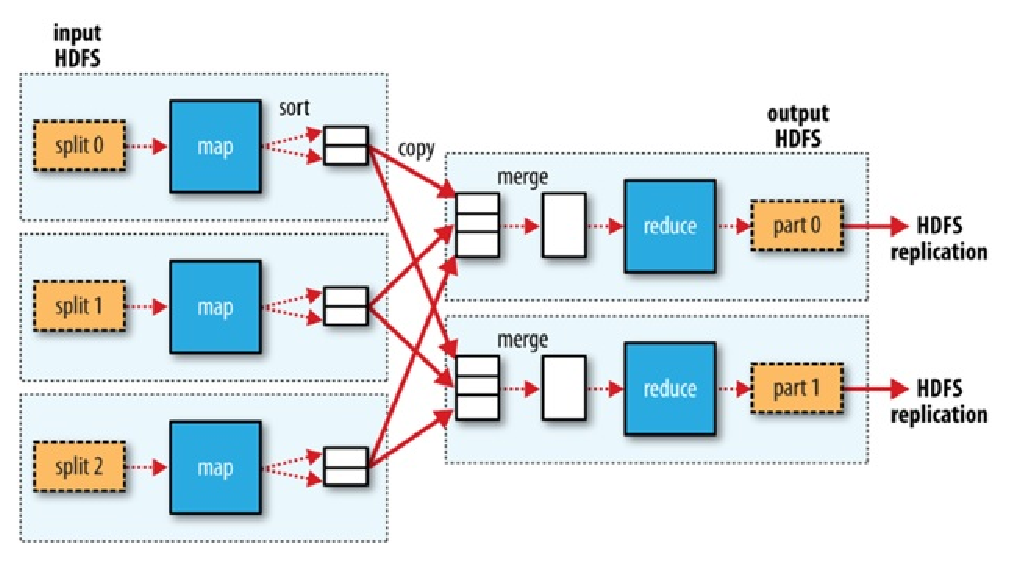
\includegraphics[keepaspectratio=true,scale=0.75]
                        {figuras/figura5.eps}
                    \caption[Fluxo de dados em um \textit{MapReduce} com múltiplas tarefas de redução]
                    {Fluxo de dados em um \textit{MapReduce} com múltiplas tarefas de redução
                    \protect \linebreak Fonte: \citeonline{white2015}}
                    \label{figura5}
            \end{figure}

            \subsubsection{Arquitetura do MapReduce}

                Para entendermos a arquitetura do \textit{MapReduce}, vamos passar por algumas fases do processo.
                O \textit{Hadoop} divide a entrada de dados dos \textit{MapReduce jobs} em pedaços de tamanho fixo
                chamados \textit{input splits}. O \textit{Hadoop} então cria um \textit{map task} para cada cada \textit{split},
                e roda as configurações definidas pelo usuário na função \textit{map} para cada registro do \textit{split}.
                Com vários \textit{splits} significa que o tempo de processamento de cada \textit{split} é menor
                comparado ao tempo de processamento de um \textit{split} completo. Se estamos processando os
                \textit{splits} em paralelo, o balanceamento de carga é mais efetivo, já quando os \textit{splits} são
                pequenos, uma máquina rápida irá processar mais \textit{splits} comparado a uma máquina lenta
                \cite{white2015}.

                A invocação do \textit{map} é distribuída, ao longo de várias máquinas automaticamente particionando
                os dados de entrada em intervalor de vários \textit{splits}. Os \textit{input splits} podem ser processados
                em paralelo em diferentes máquinas. As invocações do \textit{reducer} são distribuídas pelo
                particionamento do espaço da chave intermediária em vários \textit{splits} usando a função de
                particionamento. O número de partições e de funções de particionamento são especificadas pelo usuário.

                Na figura \ref{figura6} abaixo temos a visualização do fluxo geral das operações do \textit{MapReduce}.
                Quando um programa chama as funções de \textit{MapReduce}, a seguinte sequência de ações ocorre.
                A biblioteca do \textit{MapReduce} no programa do usuário divide os arquivos de entrada em vários
                \textit{splits} tipicamente de 64-128MB por \textit{split}. Então ele inicia várias instancias do programa
                no \textit{cluster} indicado \cite{dean2008}.

                De acordo com \citeonline{dean2008}, uma das instancias do programa (o \textit{master}) é especial.
                O resto são trabalhadores que terão tarefas designadas pelo \textit{master}. Existem vários \textit{map tasks}
                e  \textit{reduce tasks} a serem atribuídos. O \textit{master} decide os trabalhadores, que estão ociosos,
                para atribuir a cada um deles um \textit{map task} e um \textit{reduce task} que serão processados. O
                trabalhador que foi atribuído ao \textit{map task} irá ler o conteúdo do \textit{input split} correspondente.
                Ele analisa o par de \{chave,valor\} dos dados de entrada e repassa cada par a função de \textit{map}
                definida pelo usuário. Os pares de {chave,valor} intermediários serão produzidos pela função de \textit{map}
                que está armazenada em \textit{buffer} na memória.

                Tanto para \citeonline{dean2008} quanto para \citeonline{white2015}, ambos explicam que periodicamente,
                os pares que estão em \textit{buffer} são escritos no disco local, e particionados em regiões pela função de
                particionamento. A localização desses pares em \textit{buffer} no disco local é repassada ao \textit{master}
                que irá se responsabilizar pelo repasse dessas localizações aos \textit{reduce workers}. Quando um \textit{
                reduce worker} é notificado pelo \textit{master} sobre a localização, ele usa um recursos chamado \textit{
                Remote Procedure Calls} (RPC) para ler os dados do \textit{buffer} do disco local dos \textit{map workers}.
                Então depois que o \textit{reduce worker} lê todos os dados intermediários da partição, ele organiza por
                chave intermediária para que todas as ocorrências da mesma chave sejam agrupadas. A organização é
                necessária por causa que diferentes chaves são mapeadas para o mesmo \textit{reduce task}. E se esse
                agrupamento de dados intermediários for muito grande para caber em memória, uma organização externa
                será necessária.

                O \textit{reduce worker} itera sobre os dados intermediários organizados e para cada chave intermediária
                única encontrada, ele repassa a chave e o intervalo de valores intermediários correspondentes a função de
                \textit{reduce} do usuário. A saída da função \textit{reduce} é acrescentada ao final do arquivo de saída
                para essa partição do \textit{reduce}. Quando todos os \textit{map tasks} e \textit{reduce tasks} forem
                completados, o \textit{master} acorda a aplicação. Nesse ponto o \textit{MapReduce} repassa o retorno
                da aplicação para o código do usuário \cite{dean2008}.

                \begin{figure}[ht!]
                    \centering
                    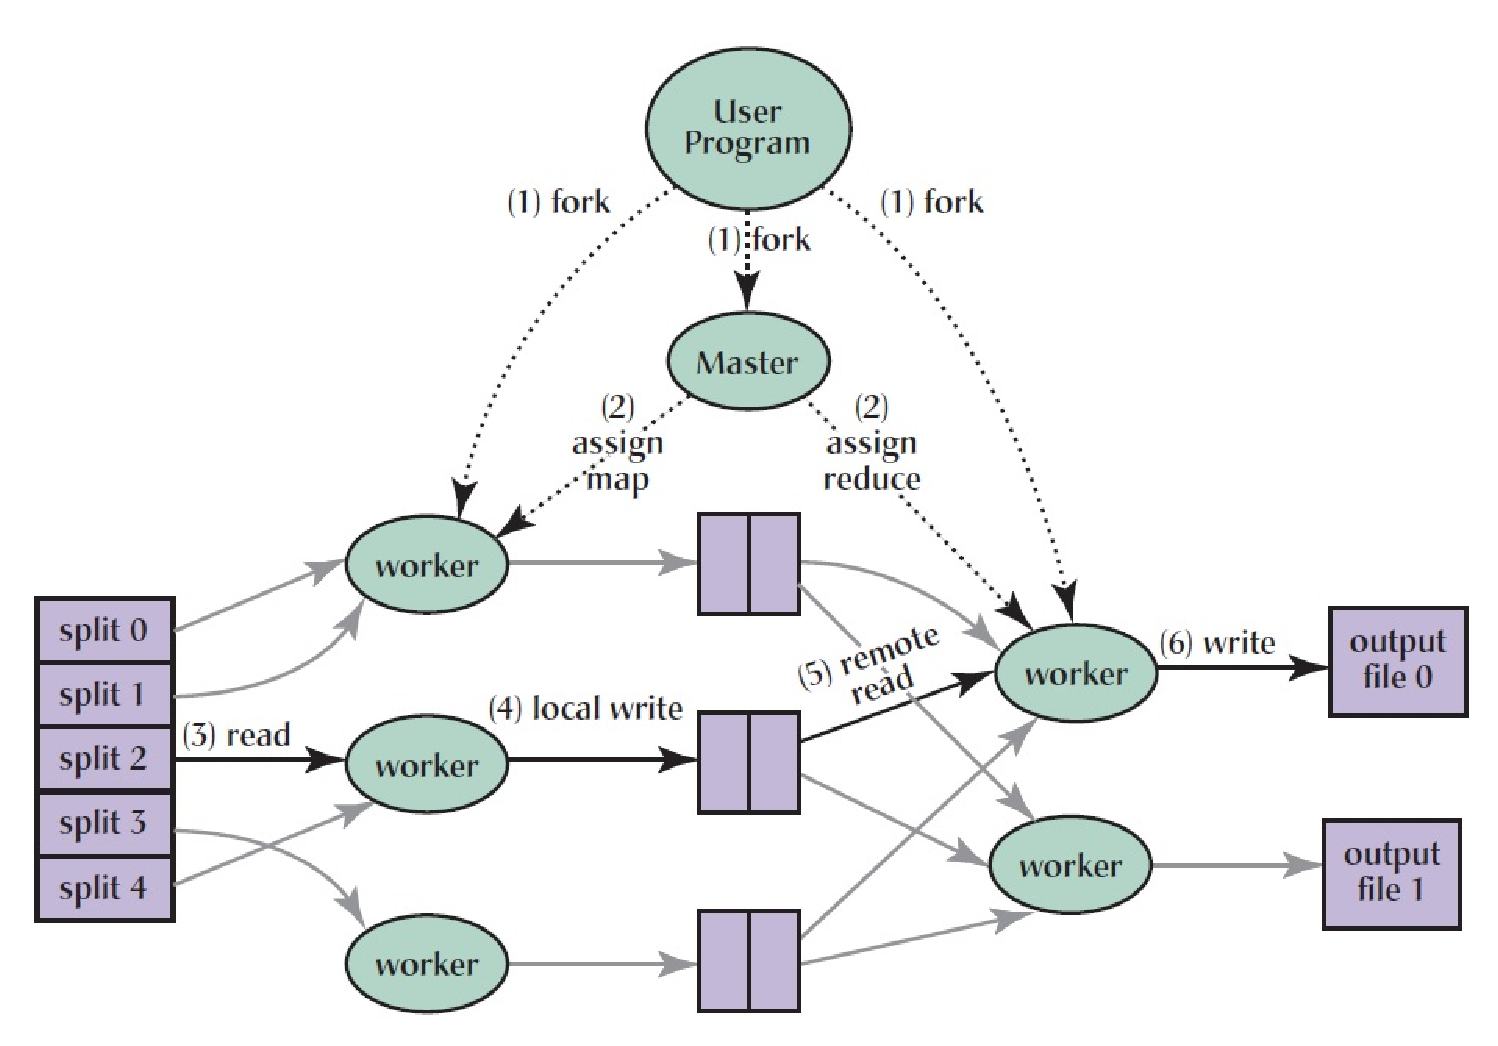
\includegraphics[keepaspectratio=true,scale=0.5]
                        {figuras/figura6.eps}
                    \caption[Fluxo de dados do processo de execução do \textit{MapReduce}]
                    {Fluxo de dados do processo de execução do \textit{MapReduce}
                    \protect \linebreak Fonte: \citeonline{dean2008}}
                    \label{figura6}
                \end{figure}

        \subsection{YARN}

            Apache YARN (\textit{Yet Another Resource Negotiator}) é um sistema de gerenciamento de recursos para
            um \textit{cluster Hadoop}. O YARN foi introduzido nas novas versões do \textit{Hadoop} 2.x para melhorar
            a implementação do \textit{MapReduce}, mas em geral é usado para suporta outros paradigmas da
            computação distribuída também \cite{yarnapache}.

            Segundo as explicações de \citeonline{vavilapalli2013}, o YARN provê dois tipos de serviços essenciais que são
            executados em \textit{background}, o \textit{resource manager} para gerenciamento do uso de recursos ao
            longo do \textit{cluster}, e os \textit{node managers} que são executados em todos os \textit{nodes} de um
            \textit{cluster}, para monitorar os \textit{containers}. O \textit{container} executa um processo de aplicação
            específica com restrição a uma série de recursos (memória, CPU e etc.).

            \begin{figure}[ht!]
                        \centering
                        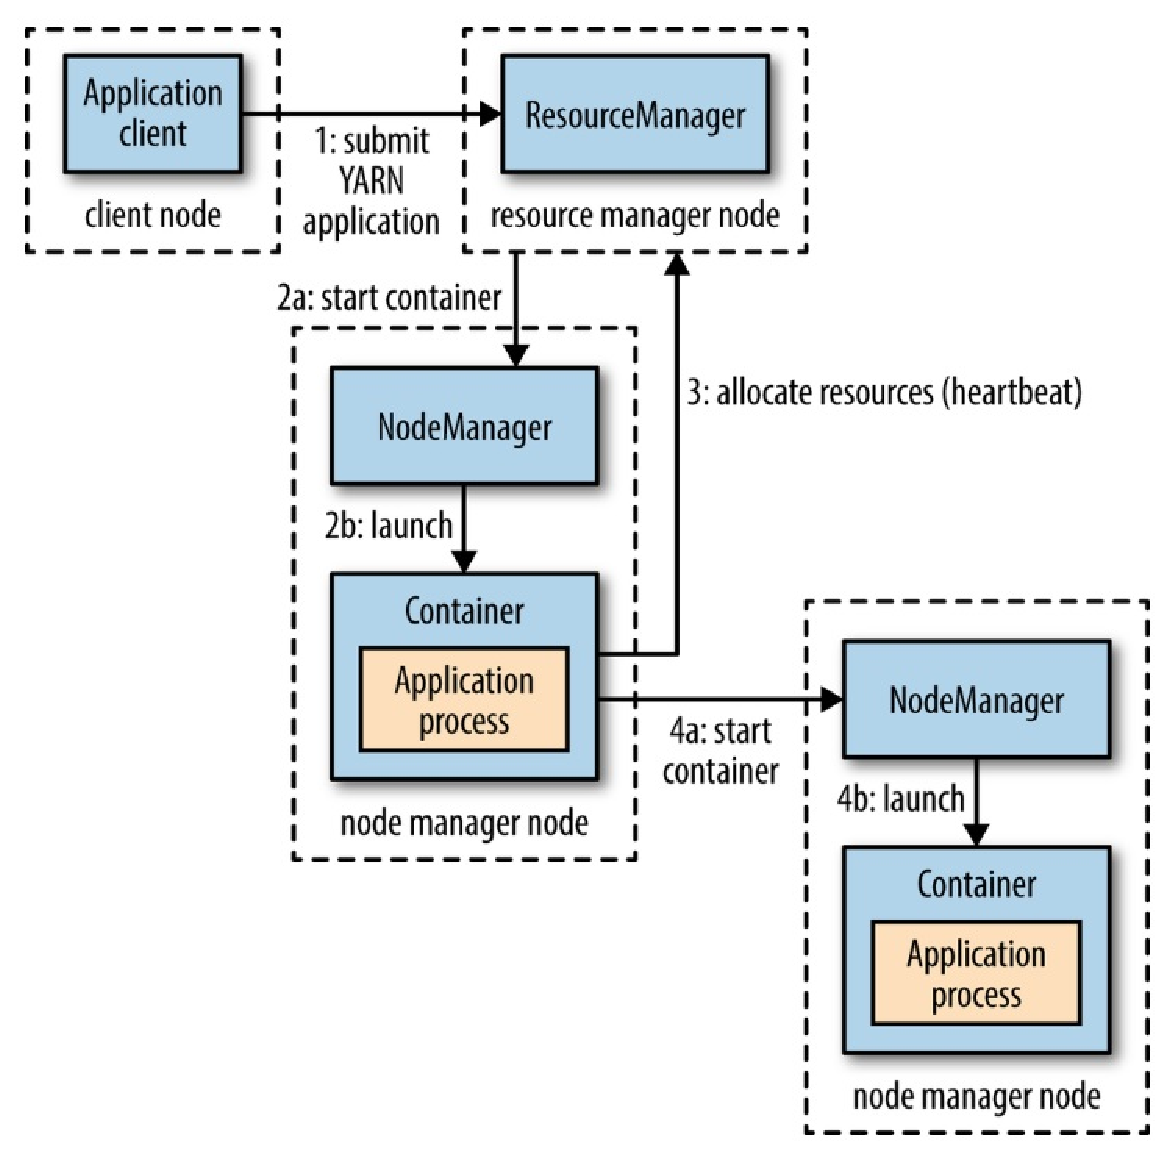
\includegraphics[keepaspectratio=true,scale=0.5]
                            {figuras/figura7.eps}
                        \caption[Anatomia de um processo em execução no YARN]{Anatomia de um processo em execução no YARN
                        \protect \linebreak Fonte: \citeonline{white2015}}
                        \label{figura7}
            \end{figure}

            Para executar uma aplicação no YARN, o \textit{client} chama o \textit{resource manager} e pede para executar
            o \textit{application master process}. O \textit{resource manager} então procura um \textit{node manager} que
            possa executar o \textit{application master} em um \textit{container}. A execução do \textit{application master}
            vai depender do comportamento da aplicação \cite{vavilapalli2013}. Na figura \ref{figura7} temos a arquitetura de
            execução de um \textit{application master} no YARN, então vários passos são executados até chegar a melhor
            otimização possível de recursos em paralelo com as outros \textit{jobs} em execução.

            \subsubsection{Requisição de Recursos}

                O YARN possui um modelo de flexibilidade para realização de requisição de recursos. Uma requisição para um
                intervalor de \textit{containers} pode ser expressa por um percentual dos recursos computacionais requeridos
                para cada container, bem como as restrições de localidades para cada \textit{container} naquela determinada
                requisição \cite{white2015}.

                A localidade é crítica em garantir que o algoritmo de processamento de dados distribuídos use a banda do
                \textit{cluster} de forma eficiente, então o YARN permite que a aplicação especifique as restrições de
                localidade para as requisições dos \textit{containers} \cite{vavilapalli2013}. Requisições de localidade
                podem ser usadas para requisitar um \textit{container} em um \textit{node, rack} ou qualquer outro lugar
                especifico fora do \textit{rack} \cite{white2015}.

            \subsubsection{Tempo de Vida da Aplicação}

                O tempo de vida de uma aplicação YARN pode variar bastante de um pequeno ciclo de apenas alguns segundos
                a um grande ciclo que possui um tempo de execução de dias ou meses. A eficiência de um tempo de vida da
                aplicação recai na categorização das aplicações em termos de como realizar o mapeamento dos \textit{jobs}
                que o usuário executa \cite{yarnapache}.

                O caso mais simples é a de uma aplicação do \textit{job} de usuário, que é a mesma aproximação utilizadas pelas
                \textit{tasks} do \textit{MapReduce}. O segundo modelo é a de rodar uma aplicação por fluxo ou por sessão de
                usuário. Essa aproximação pode ser mais eficiente que a primeira, já que os \textit{containers} podem ser reusados
                entre os \textit{jobs}, e ainda existe o potencial de \textit{cache} intermediário entre os \textit{jobs}
                \cite{yarnapache}.

            \subsubsection{Tipos de Agendamento}

                O objetivo do YARN está como um gerenciador de recursos que irá realocar os recursos para as aplicações de acordo
                com uma política definida. Agendamento em geral é um problema complexo, e não existe uma política ideal, por isso
                que o YARN disponibiliza escolhas para gerenciamento do agendamento de recursos e configurações das políticas de
                agendamento \cite{vavilapalli2013}.

                O \citeonline{white2015} elabora sobre o YARN, explicando que ele disponibiliza três tipos de agendamento de recursos,
                que são o \textit{First In First Out} (FIFO), \textit{Capacity} e o \textit{Fair Schedulers}. O agendamento usando FIFO
                organiza as aplicações em uma fila por ordem de submissão em que o primeiro a entrar é o primeiro a sair. Requisições
                para a primeira aplicação, que para \citeonline{white2015}, são alocadas primeiramente na fila, depois que as requisições
                forem satisfeitas, a próxima aplicação é executada e assim por diante.

                De acordo com \citeonline{white2015} e com a complementação de \citeonline{vavilapalli2013}, ambos relatam que para o
                agendamento \textit{Capacity}, uma fila dedicada é criada separadamente que irá permitir que pequenos \textit{jobs}
                iniciem assim que possível após terem sido submetidos, só que esse tipo de configuração possui um custo de utilização
                da capacidade do \textit{cluster} quase todo já que a capacidade da fila é reservada para \textit{jobs} que estão
                naquela fila. Isso significa que \textit{jobs} maiores irão terminar mais tarde, com essa determinada configuração.

                O \textit{Fair Scheduler} é uma configuração em que não existe a necessidade de reservar um percentual da
                capacidade, desde que os recursos sejam dinamicamente balanceados entre os \textit{jobs} que estão sendo executados.
                Só depois que um \textit{job} grande for executado, que esse será o único \textit{job} executado no momento, então ele
                terá acesso a todos os recursos no cluster. Quando um \textit{job} pequeno inicia, os recursos do cluster serão alocados de
                forma justa, e assim por diante de acordo com o tamanho do \textit{job}, logo cada \textit{job} terá de dividir os recursos de
                forma justa para os outros \textit{jobs} que estão sendo executados simultaneamente \cite{white2015}.

                \begin{figure}[ht!]
                        \centering
                        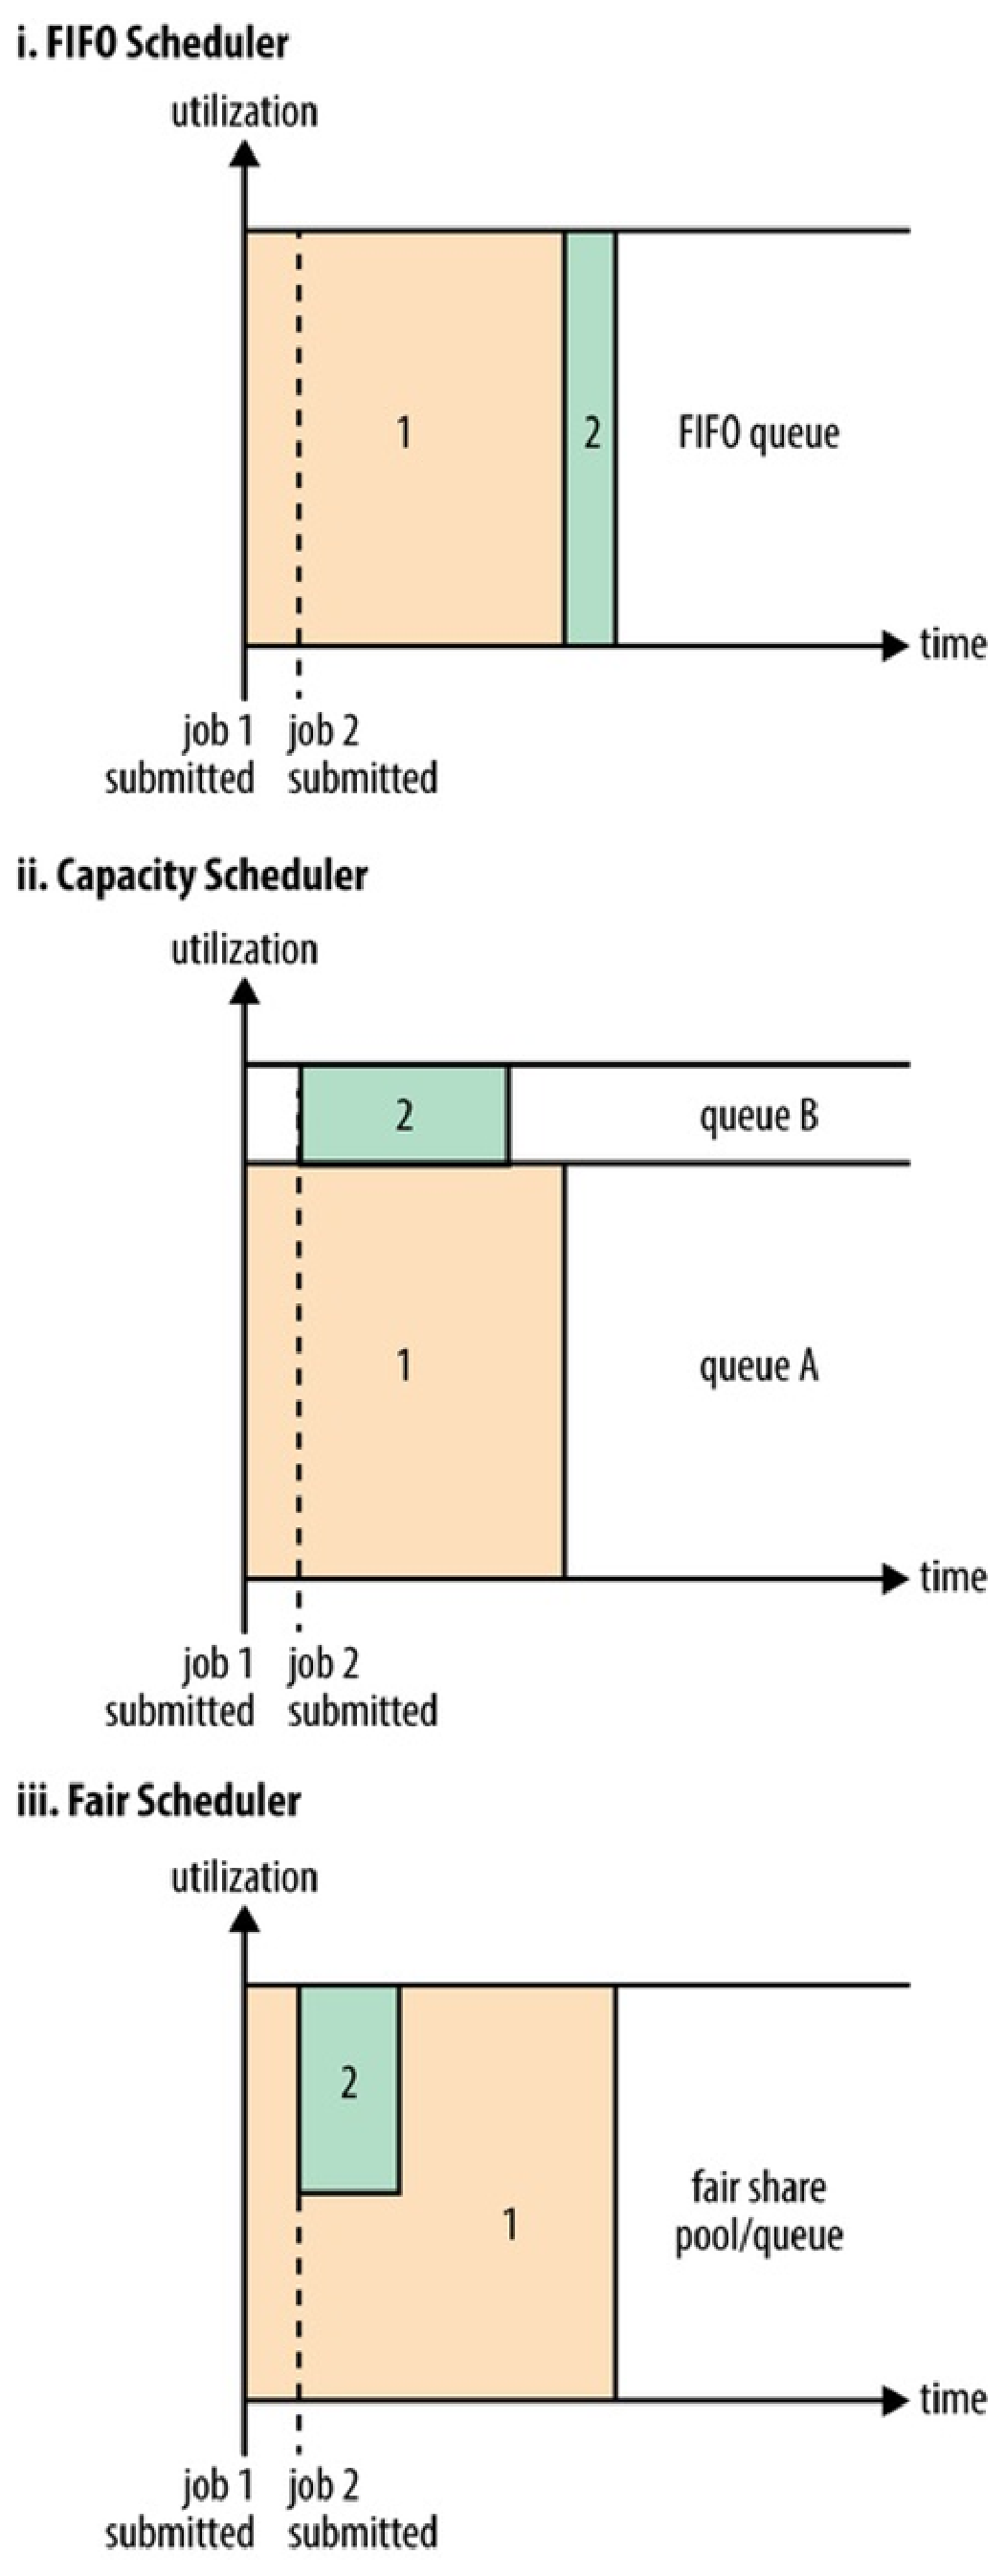
\includegraphics[keepaspectratio=true,scale=0.30]
                            {figuras/figura8.eps}
                        \caption[Opções de agendamento do YARN]{Opções de agendamento do YARN
                        \protect \linebreak Fonte: \citeonline{white2015}}
                        \label{figura8}
                 \end{figure}





    \section{HBase}

    \section{Spark}

    \section{Impala}



